\documentclass[twoside]{book}

% Packages required by doxygen
\usepackage{fixltx2e}
\usepackage{calc}
\usepackage{doxygen}
\usepackage[export]{adjustbox} % also loads graphicx
\usepackage{graphicx}
\usepackage[utf8]{inputenc}
\usepackage{makeidx}
\usepackage{multicol}
\usepackage{multirow}
\PassOptionsToPackage{warn}{textcomp}
\usepackage{textcomp}
\usepackage[nointegrals]{wasysym}
\usepackage[table]{xcolor}

% Font selection
\usepackage[T1]{fontenc}
\usepackage[scaled=.90]{helvet}
\usepackage{courier}
\usepackage{amssymb}
\usepackage{sectsty}
\renewcommand{\familydefault}{\sfdefault}
\allsectionsfont{%
  \fontseries{bc}\selectfont%
  \color{darkgray}%
}
\renewcommand{\DoxyLabelFont}{%
  \fontseries{bc}\selectfont%
  \color{darkgray}%
}
\newcommand{\+}{\discretionary{\mbox{\scriptsize$\hookleftarrow$}}{}{}}

% Page & text layout
\usepackage{geometry}
\geometry{%
  a4paper,%
  top=2.5cm,%
  bottom=2.5cm,%
  left=2.5cm,%
  right=2.5cm%
}
\tolerance=750
\hfuzz=15pt
\hbadness=750
\setlength{\emergencystretch}{15pt}
\setlength{\parindent}{0cm}
\setlength{\parskip}{3ex plus 2ex minus 2ex}
\makeatletter
\renewcommand{\paragraph}{%
  \@startsection{paragraph}{4}{0ex}{-1.0ex}{1.0ex}{%
    \normalfont\normalsize\bfseries\SS@parafont%
  }%
}
\renewcommand{\subparagraph}{%
  \@startsection{subparagraph}{5}{0ex}{-1.0ex}{1.0ex}{%
    \normalfont\normalsize\bfseries\SS@subparafont%
  }%
}
\makeatother

% Headers & footers
\usepackage{fancyhdr}
\pagestyle{fancyplain}
\fancyhead[LE]{\fancyplain{}{\bfseries\thepage}}
\fancyhead[CE]{\fancyplain{}{}}
\fancyhead[RE]{\fancyplain{}{\bfseries\leftmark}}
\fancyhead[LO]{\fancyplain{}{\bfseries\rightmark}}
\fancyhead[CO]{\fancyplain{}{}}
\fancyhead[RO]{\fancyplain{}{\bfseries\thepage}}
\fancyfoot[LE]{\fancyplain{}{}}
\fancyfoot[CE]{\fancyplain{}{}}
\fancyfoot[RE]{\fancyplain{}{\bfseries\scriptsize Generated by Doxygen }}
\fancyfoot[LO]{\fancyplain{}{\bfseries\scriptsize Generated by Doxygen }}
\fancyfoot[CO]{\fancyplain{}{}}
\fancyfoot[RO]{\fancyplain{}{}}
\renewcommand{\footrulewidth}{0.4pt}
\renewcommand{\chaptermark}[1]{%
  \markboth{#1}{}%
}
\renewcommand{\sectionmark}[1]{%
  \markright{\thesection\ #1}%
}

% Indices & bibliography
\usepackage{natbib}
\usepackage[titles]{tocloft}
\setcounter{tocdepth}{3}
\setcounter{secnumdepth}{5}
\makeindex

% Hyperlinks (required, but should be loaded last)
\usepackage{ifpdf}
\ifpdf
  \usepackage[pdftex,pagebackref=true]{hyperref}
\else
  \usepackage[ps2pdf,pagebackref=true]{hyperref}
\fi
\hypersetup{%
  colorlinks=true,%
  linkcolor=blue,%
  citecolor=blue,%
  unicode%
}

% Custom commands
\newcommand{\clearemptydoublepage}{%
  \newpage{\pagestyle{empty}\cleardoublepage}%
}

\usepackage{caption}
\captionsetup{labelsep=space,justification=centering,font={bf},singlelinecheck=off,skip=4pt,position=top}

%===== C O N T E N T S =====

\begin{document}

% Titlepage & ToC
\hypersetup{pageanchor=false,
             bookmarksnumbered=true,
             pdfencoding=unicode
            }
\pagenumbering{alph}
\begin{titlepage}
\vspace*{7cm}
\begin{center}%
{\Large Image\+Recognition \\[1ex]\large 0.\+1 }\\
\vspace*{1cm}
{\large Generated by Doxygen 1.8.13}\\
\end{center}
\end{titlepage}
\clearemptydoublepage
\pagenumbering{roman}
\tableofcontents
\clearemptydoublepage
\pagenumbering{arabic}
\hypersetup{pageanchor=true}

%--- Begin generated contents ---
\chapter{Namespace Index}
\section{Namespace List}
Here is a list of all namespaces with brief descriptions\+:\begin{DoxyCompactList}
\item\contentsline{section}{\hyperlink{namespace_controller}{Controller} }{\pageref{namespace_controller}}{}
\item\contentsline{section}{\hyperlink{namespace_controller_1_1_controlador}{Controller.\+Controlador} }{\pageref{namespace_controller_1_1_controlador}}{}
\item\contentsline{section}{\hyperlink{namespace_controller_1_1_controlador_prueba_unitaria}{Controller.\+Controlador\+Prueba\+Unitaria} }{\pageref{namespace_controller_1_1_controlador_prueba_unitaria}}{}
\item\contentsline{section}{\hyperlink{namespace_controller_1_1_gestor_general}{Controller.\+Gestor\+General} }{\pageref{namespace_controller_1_1_gestor_general}}{}
\item\contentsline{section}{\hyperlink{namespace_controller_1_1_gestor_sujeto}{Controller.\+Gestor\+Sujeto} }{\pageref{namespace_controller_1_1_gestor_sujeto}}{}
\item\contentsline{section}{\hyperlink{namespace_controller_1_1main}{Controller.\+main} }{\pageref{namespace_controller_1_1main}}{}
\item\contentsline{section}{\hyperlink{namespacedocstring}{docstring} \\*Created on Aug 16, 2017 }{\pageref{namespacedocstring}}{}
\end{DoxyCompactList}

\chapter{Hierarchical Index}
\section{Class Hierarchy}
This inheritance list is sorted roughly, but not completely, alphabetically\+:\begin{DoxyCompactList}
\item object\begin{DoxyCompactList}
\item \contentsline{section}{Controller.\+Controlador.\+Controlador}{\pageref{class_controller_1_1_controlador_1_1_controlador}}{}
\item \contentsline{section}{Controller.\+Gestor\+General.\+Gestor\+General}{\pageref{class_controller_1_1_gestor_general_1_1_gestor_general}}{}
\begin{DoxyCompactList}
\item \contentsline{section}{Controller.\+Gestor\+Sujeto.\+Gestor\+Sujeto}{\pageref{class_controller_1_1_gestor_sujeto_1_1_gestor_sujeto}}{}
\end{DoxyCompactList}
\item \contentsline{section}{Model.\+Sujeto.\+Sujeto}{\pageref{class_model_1_1_sujeto_1_1_sujeto}}{}
\end{DoxyCompactList}
\item Test\+Case\begin{DoxyCompactList}
\item \contentsline{section}{Controller.\+Controlador\+Prueba\+Unitaria.\+Controlador\+Test}{\pageref{class_controller_1_1_controlador_prueba_unitaria_1_1_controlador_test}}{}
\end{DoxyCompactList}
\end{DoxyCompactList}

\chapter{Class Index}
\section{Class List}
Here are the classes, structs, unions and interfaces with brief descriptions\+:\begin{DoxyCompactList}
\item\contentsline{section}{\hyperlink{class_controller_1_1_controlador_1_1_controlador}{Controller.\+Controlador.\+Controlador} \\*Clase controlador }{\pageref{class_controller_1_1_controlador_1_1_controlador}}{}
\item\contentsline{section}{\hyperlink{class_controller_1_1_gestor_general_1_1_gestor_general}{Controller.\+Gestor\+General.\+Gestor\+General} }{\pageref{class_controller_1_1_gestor_general_1_1_gestor_general}}{}
\item\contentsline{section}{\hyperlink{class_controller_1_1_gestor_sujeto_1_1_gestor_sujeto}{Controller.\+Gestor\+Sujeto.\+Gestor\+Sujeto} }{\pageref{class_controller_1_1_gestor_sujeto_1_1_gestor_sujeto}}{}
\end{DoxyCompactList}

\chapter{File Index}
\section{File List}
Here is a list of all files with brief descriptions\+:\begin{DoxyCompactList}
\item\contentsline{section}{Controller/\hyperlink{_controller_2____init_____8py}{\+\_\+\+\_\+init\+\_\+\+\_\+.\+py} }{\pageref{_controller_2____init_____8py}}{}
\item\contentsline{section}{Controller/\hyperlink{_controlador_8py}{Controlador.\+py} }{\pageref{_controlador_8py}}{}
\item\contentsline{section}{Controller/\hyperlink{_controlador_prueba_unitaria_8py}{Controlador\+Prueba\+Unitaria.\+py} }{\pageref{_controlador_prueba_unitaria_8py}}{}
\item\contentsline{section}{Controller/\hyperlink{_gestor_general_8py}{Gestor\+General.\+py} }{\pageref{_gestor_general_8py}}{}
\item\contentsline{section}{Controller/\hyperlink{_gestor_sujeto_8py}{Gestor\+Sujeto.\+py} }{\pageref{_gestor_sujeto_8py}}{}
\item\contentsline{section}{Controller/\hyperlink{main_8py}{main.\+py} }{\pageref{main_8py}}{}
\item\contentsline{section}{Model/\hyperlink{_model_2____init_____8py}{\+\_\+\+\_\+init\+\_\+\+\_\+.\+py} }{\pageref{_model_2____init_____8py}}{}
\item\contentsline{section}{Model/\hyperlink{_sujeto_8py}{Sujeto.\+py} }{\pageref{_sujeto_8py}}{}
\item\contentsline{section}{View/\hyperlink{_view_2____init_____8py}{\+\_\+\+\_\+init\+\_\+\+\_\+.\+py} }{\pageref{_view_2____init_____8py}}{}
\item\contentsline{section}{View/\hyperlink{_server_8py}{Server.\+py} }{\pageref{_server_8py}}{}
\end{DoxyCompactList}

\chapter{Namespace Documentation}
\hypertarget{namespace_controller}{}\section{Controller Namespace Reference}
\label{namespace_controller}\index{Controller@{Controller}}
\subsection*{Namespaces}
\begin{DoxyCompactItemize}
\item 
 \hyperlink{namespace_controller_1_1_controlador}{Controlador}
\item 
 \hyperlink{namespace_controller_1_1_controlador_prueba_unitaria}{Controlador\+Prueba\+Unitaria}
\item 
 \hyperlink{namespace_controller_1_1_gestor_general}{Gestor\+General}
\item 
 \hyperlink{namespace_controller_1_1_gestor_sujeto}{Gestor\+Sujeto}
\item 
 \hyperlink{namespace_controller_1_1main}{main}
\end{DoxyCompactItemize}

\hypertarget{namespace_controller_1_1_controlador}{}\section{Controller.\+Controlador Namespace Reference}
\label{namespace_controller_1_1_controlador}\index{Controller.\+Controlador@{Controller.\+Controlador}}
\subsection*{Classes}
\begin{DoxyCompactItemize}
\item 
class \hyperlink{class_controller_1_1_controlador_1_1_controlador}{Controlador}
\begin{DoxyCompactList}\small\item\em Clase controlador. \end{DoxyCompactList}\end{DoxyCompactItemize}

\hypertarget{namespace_controller_1_1_controlador_prueba_unitaria}{}\section{Controller.\+Controlador\+Prueba\+Unitaria Namespace Reference}
\label{namespace_controller_1_1_controlador_prueba_unitaria}\index{Controller.\+Controlador\+Prueba\+Unitaria@{Controller.\+Controlador\+Prueba\+Unitaria}}
\subsection*{Classes}
\begin{DoxyCompactItemize}
\item 
class \hyperlink{class_controller_1_1_controlador_prueba_unitaria_1_1_controlador_test}{Controlador\+Test}
\end{DoxyCompactItemize}


\subsection{Detailed Description}
\begin{DoxyVerb}Created on Aug 19, 2017

@author: HP
\end{DoxyVerb}
 
\hypertarget{namespace_controller_1_1_gestor_general}{}\section{Controller.\+Gestor\+General Namespace Reference}
\label{namespace_controller_1_1_gestor_general}\index{Controller.\+Gestor\+General@{Controller.\+Gestor\+General}}
\subsection*{Classes}
\begin{DoxyCompactItemize}
\item 
class \hyperlink{class_controller_1_1_gestor_general_1_1_gestor_general}{Gestor\+General}
\end{DoxyCompactItemize}


\subsection{Detailed Description}
\begin{DoxyVerb}Created on Aug 16, 2017

@author: HP
\end{DoxyVerb}
 
\hypertarget{namespace_controller_1_1_gestor_sujeto}{}\section{Controller.\+Gestor\+Sujeto Namespace Reference}
\label{namespace_controller_1_1_gestor_sujeto}\index{Controller.\+Gestor\+Sujeto@{Controller.\+Gestor\+Sujeto}}
\subsection*{Classes}
\begin{DoxyCompactItemize}
\item 
class \hyperlink{class_controller_1_1_gestor_sujeto_1_1_gestor_sujeto}{Gestor\+Sujeto}
\begin{DoxyCompactList}\small\item\em Clase \hyperlink{class_controller_1_1_gestor_sujeto_1_1_gestor_sujeto}{Gestor\+Sujeto}. \end{DoxyCompactList}\end{DoxyCompactItemize}

\hypertarget{namespace_controller_1_1main}{}\section{Controller.\+main Namespace Reference}
\label{namespace_controller_1_1main}\index{Controller.\+main@{Controller.\+main}}
\subsection*{Variables}
\begin{DoxyCompactItemize}
\item 
\hyperlink{namespace_controller_1_1main_afde056e3ffb39cf4210266e4a3c724ec}{script\+Dir} = os.\+path.\+dirname(\+\_\+\+\_\+file\+\_\+\+\_\+)
\item 
int \hyperlink{namespace_controller_1_1main_a551a13a2be12ee8db7e027437ded21e7}{contador} = 0
\item 
list \hyperlink{namespace_controller_1_1main_adc676146e1b9b81c62c7d962e6a09b73}{dirs} = \mbox{[}d for d in os.\+listdir(\textquotesingle{}../Images/\textquotesingle{}) if os.\+path.\+isdir(os.\+path.\+join(\textquotesingle{}../Images/\textquotesingle{}, d))\mbox{]}
\item 
\hyperlink{namespace_controller_1_1main_a6808351aab7a7dabdfde550a30c719b1}{lista} = os.\+listdir(\textquotesingle{}../Images/\textquotesingle{})
\item 
\hyperlink{namespace_controller_1_1main_ab64b1d5d85baa87feb723b5020958dc9}{numero\+Imagenes} = len(\hyperlink{namespace_controller_1_1main_a6808351aab7a7dabdfde550a30c719b1}{lista})
\item 
list \hyperlink{namespace_controller_1_1main_a4272c41c978f6d49bb441a74e2f83b97}{matriz\+Img\+Vec} = \mbox{[}\mbox{[}$\,$\mbox{]}\mbox{]}
\item 
\hyperlink{namespace_controller_1_1main_ada4e168ced647a0550eb8ae2c15e1037}{impath} = os.\+path.\+join(\hyperlink{namespace_controller_1_1main_afde056e3ffb39cf4210266e4a3c724ec}{script\+Dir},\textquotesingle{}../Images/s1/\textquotesingle{}+str(\hyperlink{namespace_controller_1_1main_a551a13a2be12ee8db7e027437ded21e7}{contador}+1)+\textquotesingle{}.pgm\textquotesingle{})
\item 
\hyperlink{namespace_controller_1_1main_adad82d87439471603c309d29ce1fcd16}{arr} = cv2.\+imread(\hyperlink{namespace_controller_1_1main_ada4e168ced647a0550eb8ae2c15e1037}{impath},0)
\item 
\hyperlink{namespace_controller_1_1main_aedd35c1d9c6106eaec585482a5020709}{flat\+\_\+arr} = arr.\+ravel()
\item 
int \hyperlink{namespace_controller_1_1main_a71a788edfd86f78336518c22203e2bc4}{y} = 1
\item 
\hyperlink{namespace_controller_1_1main_a16245faf87dfaee9eec6634fd40179c0}{m} = np.\+cov(\mbox{[}\mbox{[}1,2\mbox{]},\mbox{[}3,4\mbox{]}\mbox{]})
\end{DoxyCompactItemize}


\subsection{Variable Documentation}
\mbox{\Hypertarget{namespace_controller_1_1main_adad82d87439471603c309d29ce1fcd16}\label{namespace_controller_1_1main_adad82d87439471603c309d29ce1fcd16}} 
\index{Controller\+::main@{Controller\+::main}!arr@{arr}}
\index{arr@{arr}!Controller\+::main@{Controller\+::main}}
\subsubsection{\texorpdfstring{arr}{arr}}
{\footnotesize\ttfamily Controller.\+main.\+arr = cv2.\+imread(\hyperlink{namespace_controller_1_1main_ada4e168ced647a0550eb8ae2c15e1037}{impath},0)}

\mbox{\Hypertarget{namespace_controller_1_1main_a551a13a2be12ee8db7e027437ded21e7}\label{namespace_controller_1_1main_a551a13a2be12ee8db7e027437ded21e7}} 
\index{Controller\+::main@{Controller\+::main}!contador@{contador}}
\index{contador@{contador}!Controller\+::main@{Controller\+::main}}
\subsubsection{\texorpdfstring{contador}{contador}}
{\footnotesize\ttfamily int Controller.\+main.\+contador = 0}

\mbox{\Hypertarget{namespace_controller_1_1main_adc676146e1b9b81c62c7d962e6a09b73}\label{namespace_controller_1_1main_adc676146e1b9b81c62c7d962e6a09b73}} 
\index{Controller\+::main@{Controller\+::main}!dirs@{dirs}}
\index{dirs@{dirs}!Controller\+::main@{Controller\+::main}}
\subsubsection{\texorpdfstring{dirs}{dirs}}
{\footnotesize\ttfamily list Controller.\+main.\+dirs = \mbox{[}d for d in os.\+listdir(\textquotesingle{}../Images/\textquotesingle{}) if os.\+path.\+isdir(os.\+path.\+join(\textquotesingle{}../Images/\textquotesingle{}, d))\mbox{]}}

\mbox{\Hypertarget{namespace_controller_1_1main_aedd35c1d9c6106eaec585482a5020709}\label{namespace_controller_1_1main_aedd35c1d9c6106eaec585482a5020709}} 
\index{Controller\+::main@{Controller\+::main}!flat\+\_\+arr@{flat\+\_\+arr}}
\index{flat\+\_\+arr@{flat\+\_\+arr}!Controller\+::main@{Controller\+::main}}
\subsubsection{\texorpdfstring{flat\+\_\+arr}{flat\_arr}}
{\footnotesize\ttfamily Controller.\+main.\+flat\+\_\+arr = arr.\+ravel()}

\mbox{\Hypertarget{namespace_controller_1_1main_ada4e168ced647a0550eb8ae2c15e1037}\label{namespace_controller_1_1main_ada4e168ced647a0550eb8ae2c15e1037}} 
\index{Controller\+::main@{Controller\+::main}!impath@{impath}}
\index{impath@{impath}!Controller\+::main@{Controller\+::main}}
\subsubsection{\texorpdfstring{impath}{impath}}
{\footnotesize\ttfamily Controller.\+main.\+impath = os.\+path.\+join(\hyperlink{namespace_controller_1_1main_afde056e3ffb39cf4210266e4a3c724ec}{script\+Dir},\textquotesingle{}../Images/s1/\textquotesingle{}+str(\hyperlink{namespace_controller_1_1main_a551a13a2be12ee8db7e027437ded21e7}{contador}+1)+\textquotesingle{}.pgm\textquotesingle{})}

\mbox{\Hypertarget{namespace_controller_1_1main_a6808351aab7a7dabdfde550a30c719b1}\label{namespace_controller_1_1main_a6808351aab7a7dabdfde550a30c719b1}} 
\index{Controller\+::main@{Controller\+::main}!lista@{lista}}
\index{lista@{lista}!Controller\+::main@{Controller\+::main}}
\subsubsection{\texorpdfstring{lista}{lista}}
{\footnotesize\ttfamily Controller.\+main.\+lista = os.\+listdir(\textquotesingle{}../Images/\textquotesingle{})}

\mbox{\Hypertarget{namespace_controller_1_1main_a16245faf87dfaee9eec6634fd40179c0}\label{namespace_controller_1_1main_a16245faf87dfaee9eec6634fd40179c0}} 
\index{Controller\+::main@{Controller\+::main}!m@{m}}
\index{m@{m}!Controller\+::main@{Controller\+::main}}
\subsubsection{\texorpdfstring{m}{m}}
{\footnotesize\ttfamily Controller.\+main.\+m = np.\+cov(\mbox{[}\mbox{[}1,2\mbox{]},\mbox{[}3,4\mbox{]}\mbox{]})}

\mbox{\Hypertarget{namespace_controller_1_1main_a4272c41c978f6d49bb441a74e2f83b97}\label{namespace_controller_1_1main_a4272c41c978f6d49bb441a74e2f83b97}} 
\index{Controller\+::main@{Controller\+::main}!matriz\+Img\+Vec@{matriz\+Img\+Vec}}
\index{matriz\+Img\+Vec@{matriz\+Img\+Vec}!Controller\+::main@{Controller\+::main}}
\subsubsection{\texorpdfstring{matriz\+Img\+Vec}{matrizImgVec}}
{\footnotesize\ttfamily list Controller.\+main.\+matriz\+Img\+Vec = \mbox{[}\mbox{[}$\,$\mbox{]}\mbox{]}}

\mbox{\Hypertarget{namespace_controller_1_1main_ab64b1d5d85baa87feb723b5020958dc9}\label{namespace_controller_1_1main_ab64b1d5d85baa87feb723b5020958dc9}} 
\index{Controller\+::main@{Controller\+::main}!numero\+Imagenes@{numero\+Imagenes}}
\index{numero\+Imagenes@{numero\+Imagenes}!Controller\+::main@{Controller\+::main}}
\subsubsection{\texorpdfstring{numero\+Imagenes}{numeroImagenes}}
{\footnotesize\ttfamily Controller.\+main.\+numero\+Imagenes = len(\hyperlink{namespace_controller_1_1main_a6808351aab7a7dabdfde550a30c719b1}{lista})}

\mbox{\Hypertarget{namespace_controller_1_1main_afde056e3ffb39cf4210266e4a3c724ec}\label{namespace_controller_1_1main_afde056e3ffb39cf4210266e4a3c724ec}} 
\index{Controller\+::main@{Controller\+::main}!script\+Dir@{script\+Dir}}
\index{script\+Dir@{script\+Dir}!Controller\+::main@{Controller\+::main}}
\subsubsection{\texorpdfstring{script\+Dir}{scriptDir}}
{\footnotesize\ttfamily Controller.\+main.\+script\+Dir = os.\+path.\+dirname(\+\_\+\+\_\+file\+\_\+\+\_\+)}

\mbox{\Hypertarget{namespace_controller_1_1main_a71a788edfd86f78336518c22203e2bc4}\label{namespace_controller_1_1main_a71a788edfd86f78336518c22203e2bc4}} 
\index{Controller\+::main@{Controller\+::main}!y@{y}}
\index{y@{y}!Controller\+::main@{Controller\+::main}}
\subsubsection{\texorpdfstring{y}{y}}
{\footnotesize\ttfamily int Controller.\+main.\+y = 1}


\hypertarget{namespacedocstring}{}\section{docstring Namespace Reference}
\label{namespacedocstring}\index{docstring@{docstring}}


Created on Aug 16, 2017.  




\subsection{Detailed Description}
Created on Aug 16, 2017. 

\begin{DoxyAuthor}{Author}
Michael Choque 
\end{DoxyAuthor}

\chapter{Class Documentation}
\hypertarget{class_controller_1_1_controlador_1_1_controlador}{}\section{Controller.\+Controlador.\+Controlador Class Reference}
\label{class_controller_1_1_controlador_1_1_controlador}\index{Controller.\+Controlador.\+Controlador@{Controller.\+Controlador.\+Controlador}}


Clase controlador.  


Inheritance diagram for Controller.\+Controlador.\+Controlador\+:\begin{figure}[H]
\begin{center}
\leavevmode
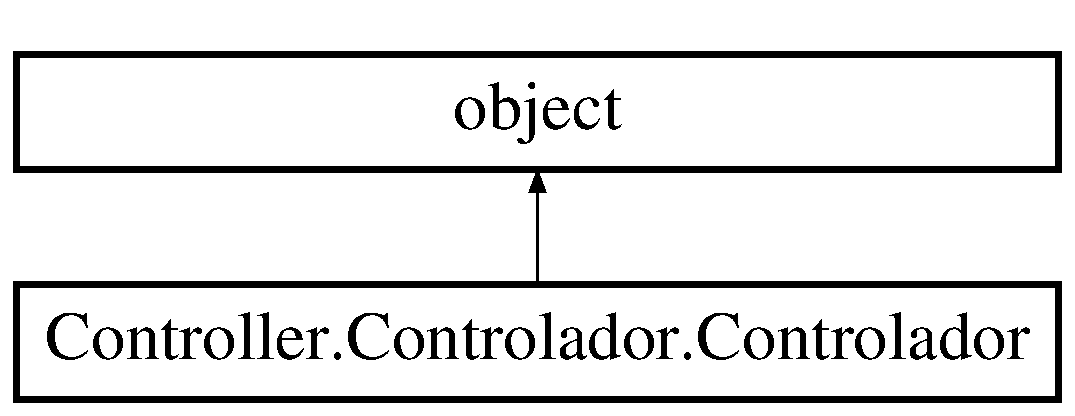
\includegraphics[height=2.000000cm]{class_controller_1_1_controlador_1_1_controlador}
\end{center}
\end{figure}
\subsection*{Public Member Functions}
\begin{DoxyCompactItemize}
\item 
def \hyperlink{class_controller_1_1_controlador_1_1_controlador_ad30f895c86fb2085fbd3b2c0a1c9f38c}{\+\_\+\+\_\+init\+\_\+\+\_\+} (self)
\begin{DoxyCompactList}\small\item\em Constructor de la clase. \end{DoxyCompactList}\item 
def \hyperlink{class_controller_1_1_controlador_1_1_controlador_a4bbeb1232cf73c6c9113e7ffda714b63}{Vectorizar\+Imagen} (self, img)
\item 
def \hyperlink{class_controller_1_1_controlador_1_1_controlador_a88254f919a6b1d7ed25e2f54b528a15c}{Definir\+Matriz\+De\+Imagenes} (self, list\+Imgs)
\item 
def \hyperlink{class_controller_1_1_controlador_1_1_controlador_a4c342a4b7f56c2f8a566cdf62030816c}{Definir\+Matriz\+De\+Covarianza} (self, matriz\+Img\+Vec)
\begin{DoxyCompactList}\small\item\em Metodo Definir\+Matriz\+De\+Covarianza. \end{DoxyCompactList}\end{DoxyCompactItemize}
\subsection*{Public Attributes}
\begin{DoxyCompactItemize}
\item 
\hyperlink{class_controller_1_1_controlador_1_1_controlador_ac7f14b4e1c0f2bf39ef0ddf2ae687898}{lista\+De\+Sujetos}
\end{DoxyCompactItemize}


\subsection{Detailed Description}
Clase controlador. 

Esta clase es la que permite la comunicacion entre los datos de la aplicacion y la interfaz de usuario 

\subsection{Constructor \& Destructor Documentation}
\mbox{\Hypertarget{class_controller_1_1_controlador_1_1_controlador_ad30f895c86fb2085fbd3b2c0a1c9f38c}\label{class_controller_1_1_controlador_1_1_controlador_ad30f895c86fb2085fbd3b2c0a1c9f38c}} 
\index{Controller\+::\+Controlador\+::\+Controlador@{Controller\+::\+Controlador\+::\+Controlador}!\+\_\+\+\_\+init\+\_\+\+\_\+@{\+\_\+\+\_\+init\+\_\+\+\_\+}}
\index{\+\_\+\+\_\+init\+\_\+\+\_\+@{\+\_\+\+\_\+init\+\_\+\+\_\+}!Controller\+::\+Controlador\+::\+Controlador@{Controller\+::\+Controlador\+::\+Controlador}}
\subsubsection{\texorpdfstring{\+\_\+\+\_\+init\+\_\+\+\_\+()}{\_\_init\_\_()}}
{\footnotesize\ttfamily def Controller.\+Controlador.\+Controlador.\+\_\+\+\_\+init\+\_\+\+\_\+ (\begin{DoxyParamCaption}\item[{}]{self }\end{DoxyParamCaption})}



Constructor de la clase. 

El constructor unicamente inicializa la lista de Sujetos en la aplicacion 

\subsection{Member Function Documentation}
\mbox{\Hypertarget{class_controller_1_1_controlador_1_1_controlador_a4c342a4b7f56c2f8a566cdf62030816c}\label{class_controller_1_1_controlador_1_1_controlador_a4c342a4b7f56c2f8a566cdf62030816c}} 
\index{Controller\+::\+Controlador\+::\+Controlador@{Controller\+::\+Controlador\+::\+Controlador}!Definir\+Matriz\+De\+Covarianza@{Definir\+Matriz\+De\+Covarianza}}
\index{Definir\+Matriz\+De\+Covarianza@{Definir\+Matriz\+De\+Covarianza}!Controller\+::\+Controlador\+::\+Controlador@{Controller\+::\+Controlador\+::\+Controlador}}
\subsubsection{\texorpdfstring{Definir\+Matriz\+De\+Covarianza()}{DefinirMatrizDeCovarianza()}}
{\footnotesize\ttfamily def Controller.\+Controlador.\+Controlador.\+Definir\+Matriz\+De\+Covarianza (\begin{DoxyParamCaption}\item[{}]{self,  }\item[{}]{matriz\+Img\+Vec }\end{DoxyParamCaption})}



Metodo Definir\+Matriz\+De\+Covarianza. 


\begin{DoxyParams}{Parameters}
{\em matriz\+Img\+Vec} & el metodo recibe una matriz de imagenes vectorizadas con la que se calculara la matriz de covarianza \\
\hline
\end{DoxyParams}
\begin{DoxyReturn}{Returns}
matriz\+Cov se devuelve la matriz de covarianza calculada 
\end{DoxyReturn}
\mbox{\Hypertarget{class_controller_1_1_controlador_1_1_controlador_a88254f919a6b1d7ed25e2f54b528a15c}\label{class_controller_1_1_controlador_1_1_controlador_a88254f919a6b1d7ed25e2f54b528a15c}} 
\index{Controller\+::\+Controlador\+::\+Controlador@{Controller\+::\+Controlador\+::\+Controlador}!Definir\+Matriz\+De\+Imagenes@{Definir\+Matriz\+De\+Imagenes}}
\index{Definir\+Matriz\+De\+Imagenes@{Definir\+Matriz\+De\+Imagenes}!Controller\+::\+Controlador\+::\+Controlador@{Controller\+::\+Controlador\+::\+Controlador}}
\subsubsection{\texorpdfstring{Definir\+Matriz\+De\+Imagenes()}{DefinirMatrizDeImagenes()}}
{\footnotesize\ttfamily def Controller.\+Controlador.\+Controlador.\+Definir\+Matriz\+De\+Imagenes (\begin{DoxyParamCaption}\item[{}]{self,  }\item[{}]{list\+Imgs }\end{DoxyParamCaption})}

\mbox{\Hypertarget{class_controller_1_1_controlador_1_1_controlador_a4bbeb1232cf73c6c9113e7ffda714b63}\label{class_controller_1_1_controlador_1_1_controlador_a4bbeb1232cf73c6c9113e7ffda714b63}} 
\index{Controller\+::\+Controlador\+::\+Controlador@{Controller\+::\+Controlador\+::\+Controlador}!Vectorizar\+Imagen@{Vectorizar\+Imagen}}
\index{Vectorizar\+Imagen@{Vectorizar\+Imagen}!Controller\+::\+Controlador\+::\+Controlador@{Controller\+::\+Controlador\+::\+Controlador}}
\subsubsection{\texorpdfstring{Vectorizar\+Imagen()}{VectorizarImagen()}}
{\footnotesize\ttfamily def Controller.\+Controlador.\+Controlador.\+Vectorizar\+Imagen (\begin{DoxyParamCaption}\item[{}]{self,  }\item[{}]{img }\end{DoxyParamCaption})}



\subsection{Member Data Documentation}
\mbox{\Hypertarget{class_controller_1_1_controlador_1_1_controlador_ac7f14b4e1c0f2bf39ef0ddf2ae687898}\label{class_controller_1_1_controlador_1_1_controlador_ac7f14b4e1c0f2bf39ef0ddf2ae687898}} 
\index{Controller\+::\+Controlador\+::\+Controlador@{Controller\+::\+Controlador\+::\+Controlador}!lista\+De\+Sujetos@{lista\+De\+Sujetos}}
\index{lista\+De\+Sujetos@{lista\+De\+Sujetos}!Controller\+::\+Controlador\+::\+Controlador@{Controller\+::\+Controlador\+::\+Controlador}}
\subsubsection{\texorpdfstring{lista\+De\+Sujetos}{listaDeSujetos}}
{\footnotesize\ttfamily Controller.\+Controlador.\+Controlador.\+lista\+De\+Sujetos}



The documentation for this class was generated from the following file\+:\begin{DoxyCompactItemize}
\item 
Controller/\hyperlink{_controlador_8py}{Controlador.\+py}\end{DoxyCompactItemize}

\hypertarget{class_controller_1_1_controlador_prueba_unitaria_1_1_controlador_test}{}\section{Controller.\+Controlador\+Prueba\+Unitaria.\+Controlador\+Test Class Reference}
\label{class_controller_1_1_controlador_prueba_unitaria_1_1_controlador_test}\index{Controller.\+Controlador\+Prueba\+Unitaria.\+Controlador\+Test@{Controller.\+Controlador\+Prueba\+Unitaria.\+Controlador\+Test}}


Clase \hyperlink{class_controller_1_1_controlador_prueba_unitaria_1_1_controlador_test}{Controlador\+Test}.  


Inheritance diagram for Controller.\+Controlador\+Prueba\+Unitaria.\+Controlador\+Test\+:\begin{figure}[H]
\begin{center}
\leavevmode
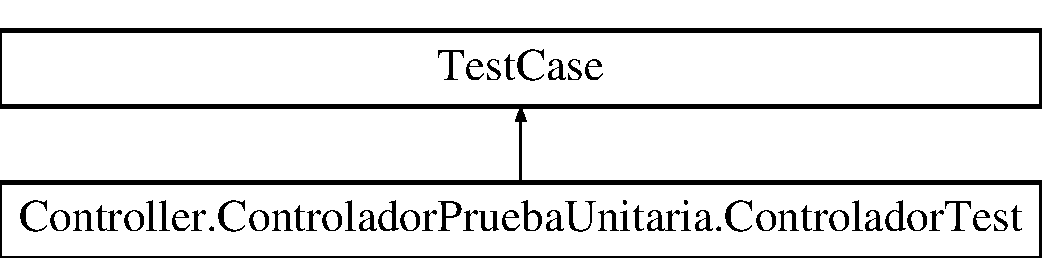
\includegraphics[height=2.000000cm]{class_controller_1_1_controlador_prueba_unitaria_1_1_controlador_test}
\end{center}
\end{figure}
\subsection*{Public Member Functions}
\begin{DoxyCompactItemize}
\item 
def \hyperlink{class_controller_1_1_controlador_prueba_unitaria_1_1_controlador_test_a2e8184870a51acab5ddda57d6ae0a6af}{set\+Up} (self)
\begin{DoxyCompactList}\small\item\em Metodo set\+Up. \end{DoxyCompactList}\item 
def \hyperlink{class_controller_1_1_controlador_prueba_unitaria_1_1_controlador_test_a0aa297aa7af4503138e4e84d3fcd40d2}{tear\+Down} (self)
\item 
def \hyperlink{class_controller_1_1_controlador_prueba_unitaria_1_1_controlador_test_ab91d55bbbbfb2b11399063e00460fed6}{test\+\_\+\+Vectorizar\+Imagen} (self)
\begin{DoxyCompactList}\small\item\em Metodo test\+\_\+\+Vectorizar\+Imagen. \end{DoxyCompactList}\item 
def \hyperlink{class_controller_1_1_controlador_prueba_unitaria_1_1_controlador_test_a149c2fe8732cf438622aefdfad75dd4a}{test\+\_\+\+Matriz\+De\+Imagenes} (self)
\begin{DoxyCompactList}\small\item\em Metodo test\+\_\+\+Matriz\+De\+Imagenes. \end{DoxyCompactList}\item 
def \hyperlink{class_controller_1_1_controlador_prueba_unitaria_1_1_controlador_test_a7bdd98073dfdcbe13627c7bee7d64f55}{test\+\_\+\+Matriz\+De\+Covarianza} (self)
\begin{DoxyCompactList}\small\item\em Metodo test\+\_\+\+Matriz\+De\+Covarianza. \end{DoxyCompactList}\end{DoxyCompactItemize}
\subsection*{Public Attributes}
\begin{DoxyCompactItemize}
\item 
\hyperlink{class_controller_1_1_controlador_prueba_unitaria_1_1_controlador_test_a2f176dc83cda878c82e90b5eed2c321a}{foo}
\end{DoxyCompactItemize}


\subsection{Detailed Description}
Clase \hyperlink{class_controller_1_1_controlador_prueba_unitaria_1_1_controlador_test}{Controlador\+Test}. 

Esta clase controla lo que tiene que ver con pruebas unitarias de la clase \hyperlink{namespace_controller_1_1_controlador}{Controlador} 

\subsection{Member Function Documentation}
\mbox{\Hypertarget{class_controller_1_1_controlador_prueba_unitaria_1_1_controlador_test_a2e8184870a51acab5ddda57d6ae0a6af}\label{class_controller_1_1_controlador_prueba_unitaria_1_1_controlador_test_a2e8184870a51acab5ddda57d6ae0a6af}} 
\index{Controller\+::\+Controlador\+Prueba\+Unitaria\+::\+Controlador\+Test@{Controller\+::\+Controlador\+Prueba\+Unitaria\+::\+Controlador\+Test}!set\+Up@{set\+Up}}
\index{set\+Up@{set\+Up}!Controller\+::\+Controlador\+Prueba\+Unitaria\+::\+Controlador\+Test@{Controller\+::\+Controlador\+Prueba\+Unitaria\+::\+Controlador\+Test}}
\subsubsection{\texorpdfstring{set\+Up()}{setUp()}}
{\footnotesize\ttfamily def Controller.\+Controlador\+Prueba\+Unitaria.\+Controlador\+Test.\+set\+Up (\begin{DoxyParamCaption}\item[{}]{self }\end{DoxyParamCaption})}



Metodo set\+Up. 

El metodo set\+Up inicializa todo lo necesario para realizar las pruebas \mbox{\Hypertarget{class_controller_1_1_controlador_prueba_unitaria_1_1_controlador_test_a0aa297aa7af4503138e4e84d3fcd40d2}\label{class_controller_1_1_controlador_prueba_unitaria_1_1_controlador_test_a0aa297aa7af4503138e4e84d3fcd40d2}} 
\index{Controller\+::\+Controlador\+Prueba\+Unitaria\+::\+Controlador\+Test@{Controller\+::\+Controlador\+Prueba\+Unitaria\+::\+Controlador\+Test}!tear\+Down@{tear\+Down}}
\index{tear\+Down@{tear\+Down}!Controller\+::\+Controlador\+Prueba\+Unitaria\+::\+Controlador\+Test@{Controller\+::\+Controlador\+Prueba\+Unitaria\+::\+Controlador\+Test}}
\subsubsection{\texorpdfstring{tear\+Down()}{tearDown()}}
{\footnotesize\ttfamily def Controller.\+Controlador\+Prueba\+Unitaria.\+Controlador\+Test.\+tear\+Down (\begin{DoxyParamCaption}\item[{}]{self }\end{DoxyParamCaption})}

\mbox{\Hypertarget{class_controller_1_1_controlador_prueba_unitaria_1_1_controlador_test_a7bdd98073dfdcbe13627c7bee7d64f55}\label{class_controller_1_1_controlador_prueba_unitaria_1_1_controlador_test_a7bdd98073dfdcbe13627c7bee7d64f55}} 
\index{Controller\+::\+Controlador\+Prueba\+Unitaria\+::\+Controlador\+Test@{Controller\+::\+Controlador\+Prueba\+Unitaria\+::\+Controlador\+Test}!test\+\_\+\+Matriz\+De\+Covarianza@{test\+\_\+\+Matriz\+De\+Covarianza}}
\index{test\+\_\+\+Matriz\+De\+Covarianza@{test\+\_\+\+Matriz\+De\+Covarianza}!Controller\+::\+Controlador\+Prueba\+Unitaria\+::\+Controlador\+Test@{Controller\+::\+Controlador\+Prueba\+Unitaria\+::\+Controlador\+Test}}
\subsubsection{\texorpdfstring{test\+\_\+\+Matriz\+De\+Covarianza()}{test\_MatrizDeCovarianza()}}
{\footnotesize\ttfamily def Controller.\+Controlador\+Prueba\+Unitaria.\+Controlador\+Test.\+test\+\_\+\+Matriz\+De\+Covarianza (\begin{DoxyParamCaption}\item[{}]{self }\end{DoxyParamCaption})}



Metodo test\+\_\+\+Matriz\+De\+Covarianza. 

Prueba del metodo Definir\+Matriz\+De\+Covarianza en la case \hyperlink{namespace_controller_1_1_controlador}{Controlador}, la prueba se realiza asegurando el tamano de la matriz (tanto filas como columnas) segun la cantidad de imagenes, la cual siempre debera de ser 10304$\ast$10304 \mbox{\Hypertarget{class_controller_1_1_controlador_prueba_unitaria_1_1_controlador_test_a149c2fe8732cf438622aefdfad75dd4a}\label{class_controller_1_1_controlador_prueba_unitaria_1_1_controlador_test_a149c2fe8732cf438622aefdfad75dd4a}} 
\index{Controller\+::\+Controlador\+Prueba\+Unitaria\+::\+Controlador\+Test@{Controller\+::\+Controlador\+Prueba\+Unitaria\+::\+Controlador\+Test}!test\+\_\+\+Matriz\+De\+Imagenes@{test\+\_\+\+Matriz\+De\+Imagenes}}
\index{test\+\_\+\+Matriz\+De\+Imagenes@{test\+\_\+\+Matriz\+De\+Imagenes}!Controller\+::\+Controlador\+Prueba\+Unitaria\+::\+Controlador\+Test@{Controller\+::\+Controlador\+Prueba\+Unitaria\+::\+Controlador\+Test}}
\subsubsection{\texorpdfstring{test\+\_\+\+Matriz\+De\+Imagenes()}{test\_MatrizDeImagenes()}}
{\footnotesize\ttfamily def Controller.\+Controlador\+Prueba\+Unitaria.\+Controlador\+Test.\+test\+\_\+\+Matriz\+De\+Imagenes (\begin{DoxyParamCaption}\item[{}]{self }\end{DoxyParamCaption})}



Metodo test\+\_\+\+Matriz\+De\+Imagenes. 

Prueba del metodo Definir\+Matriz\+De\+Imagenes en la case \hyperlink{namespace_controller_1_1_controlador}{Controlador}, la prueba se realiza asegurando el tamano de la matriz (tanto filas como columnas) segun la cantidad de imagenes \mbox{\Hypertarget{class_controller_1_1_controlador_prueba_unitaria_1_1_controlador_test_ab91d55bbbbfb2b11399063e00460fed6}\label{class_controller_1_1_controlador_prueba_unitaria_1_1_controlador_test_ab91d55bbbbfb2b11399063e00460fed6}} 
\index{Controller\+::\+Controlador\+Prueba\+Unitaria\+::\+Controlador\+Test@{Controller\+::\+Controlador\+Prueba\+Unitaria\+::\+Controlador\+Test}!test\+\_\+\+Vectorizar\+Imagen@{test\+\_\+\+Vectorizar\+Imagen}}
\index{test\+\_\+\+Vectorizar\+Imagen@{test\+\_\+\+Vectorizar\+Imagen}!Controller\+::\+Controlador\+Prueba\+Unitaria\+::\+Controlador\+Test@{Controller\+::\+Controlador\+Prueba\+Unitaria\+::\+Controlador\+Test}}
\subsubsection{\texorpdfstring{test\+\_\+\+Vectorizar\+Imagen()}{test\_VectorizarImagen()}}
{\footnotesize\ttfamily def Controller.\+Controlador\+Prueba\+Unitaria.\+Controlador\+Test.\+test\+\_\+\+Vectorizar\+Imagen (\begin{DoxyParamCaption}\item[{}]{self }\end{DoxyParamCaption})}



Metodo test\+\_\+\+Vectorizar\+Imagen. 

Prueba del metodo Vectorizar\+Imagen en la clase \hyperlink{namespace_controller_1_1_controlador}{Controlador}, la prueba se realiza asegurando que la imagen tenga el tamano correcto y confirmando el primer y ultimo pixel de a imagen (los cuales pueden variar un poco por las transformacinoes) 

\subsection{Member Data Documentation}
\mbox{\Hypertarget{class_controller_1_1_controlador_prueba_unitaria_1_1_controlador_test_a2f176dc83cda878c82e90b5eed2c321a}\label{class_controller_1_1_controlador_prueba_unitaria_1_1_controlador_test_a2f176dc83cda878c82e90b5eed2c321a}} 
\index{Controller\+::\+Controlador\+Prueba\+Unitaria\+::\+Controlador\+Test@{Controller\+::\+Controlador\+Prueba\+Unitaria\+::\+Controlador\+Test}!foo@{foo}}
\index{foo@{foo}!Controller\+::\+Controlador\+Prueba\+Unitaria\+::\+Controlador\+Test@{Controller\+::\+Controlador\+Prueba\+Unitaria\+::\+Controlador\+Test}}
\subsubsection{\texorpdfstring{foo}{foo}}
{\footnotesize\ttfamily Controller.\+Controlador\+Prueba\+Unitaria.\+Controlador\+Test.\+foo}



The documentation for this class was generated from the following file\+:\begin{DoxyCompactItemize}
\item 
Controller/\hyperlink{_controlador_prueba_unitaria_8py}{Controlador\+Prueba\+Unitaria.\+py}\end{DoxyCompactItemize}

\hypertarget{class_controller_1_1_gestor_general_1_1_gestor_general}{}\section{Controller.\+Gestor\+General.\+Gestor\+General Class Reference}
\label{class_controller_1_1_gestor_general_1_1_gestor_general}\index{Controller.\+Gestor\+General.\+Gestor\+General@{Controller.\+Gestor\+General.\+Gestor\+General}}
Inheritance diagram for Controller.\+Gestor\+General.\+Gestor\+General\+:\begin{figure}[H]
\begin{center}
\leavevmode
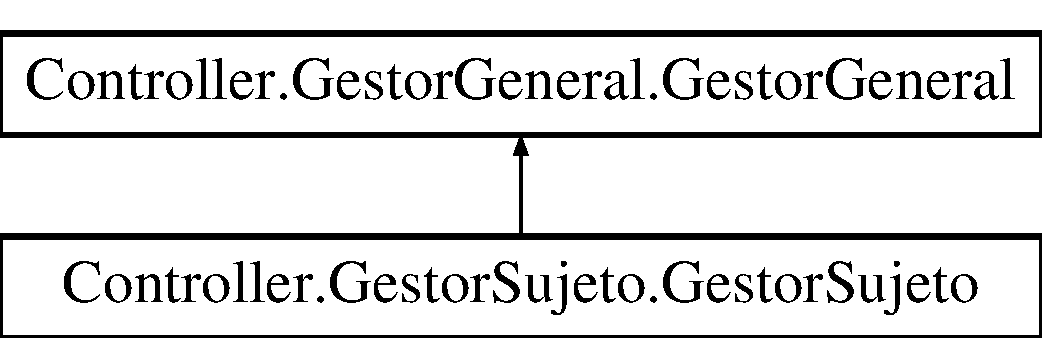
\includegraphics[height=2.000000cm]{class_controller_1_1_gestor_general_1_1_gestor_general}
\end{center}
\end{figure}


\subsection{Detailed Description}
\begin{DoxyVerb}classdocs
\end{DoxyVerb}
 

The documentation for this class was generated from the following file\+:\begin{DoxyCompactItemize}
\item 
Controller/Gestor\+General.\+py\end{DoxyCompactItemize}

\hypertarget{class_controller_1_1_gestor_sujeto_1_1_gestor_sujeto}{}\section{Controller.\+Gestor\+Sujeto.\+Gestor\+Sujeto Class Reference}
\label{class_controller_1_1_gestor_sujeto_1_1_gestor_sujeto}\index{Controller.\+Gestor\+Sujeto.\+Gestor\+Sujeto@{Controller.\+Gestor\+Sujeto.\+Gestor\+Sujeto}}
Inheritance diagram for Controller.\+Gestor\+Sujeto.\+Gestor\+Sujeto\+:\begin{figure}[H]
\begin{center}
\leavevmode
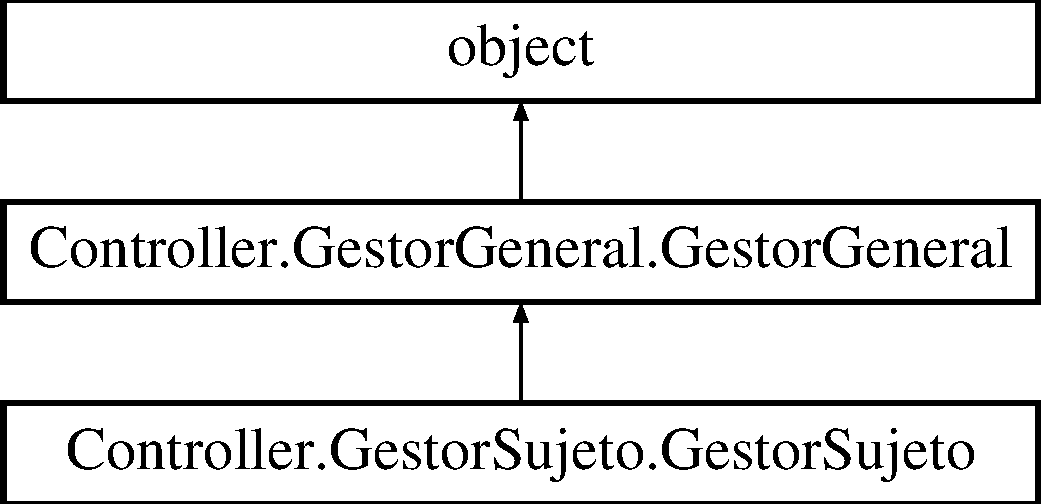
\includegraphics[height=3.000000cm]{class_controller_1_1_gestor_sujeto_1_1_gestor_sujeto}
\end{center}
\end{figure}
\subsection*{Public Member Functions}
\begin{DoxyCompactItemize}
\item 
def \hyperlink{class_controller_1_1_gestor_sujeto_1_1_gestor_sujeto_af03120d2a26ad27cf43979b059065818}{\+\_\+\+\_\+init\+\_\+\+\_\+} (self)
\end{DoxyCompactItemize}
\subsection*{Additional Inherited Members}


\subsection{Detailed Description}
\begin{DoxyVerb}classdocs
\end{DoxyVerb}
 

\subsection{Constructor \& Destructor Documentation}
\mbox{\Hypertarget{class_controller_1_1_gestor_sujeto_1_1_gestor_sujeto_af03120d2a26ad27cf43979b059065818}\label{class_controller_1_1_gestor_sujeto_1_1_gestor_sujeto_af03120d2a26ad27cf43979b059065818}} 
\index{Controller\+::\+Gestor\+Sujeto\+::\+Gestor\+Sujeto@{Controller\+::\+Gestor\+Sujeto\+::\+Gestor\+Sujeto}!\+\_\+\+\_\+init\+\_\+\+\_\+@{\+\_\+\+\_\+init\+\_\+\+\_\+}}
\index{\+\_\+\+\_\+init\+\_\+\+\_\+@{\+\_\+\+\_\+init\+\_\+\+\_\+}!Controller\+::\+Gestor\+Sujeto\+::\+Gestor\+Sujeto@{Controller\+::\+Gestor\+Sujeto\+::\+Gestor\+Sujeto}}
\subsubsection{\texorpdfstring{\+\_\+\+\_\+init\+\_\+\+\_\+()}{\_\_init\_\_()}}
{\footnotesize\ttfamily def Controller.\+Gestor\+Sujeto.\+Gestor\+Sujeto.\+\_\+\+\_\+init\+\_\+\+\_\+ (\begin{DoxyParamCaption}\item[{}]{self }\end{DoxyParamCaption})}



The documentation for this class was generated from the following file\+:\begin{DoxyCompactItemize}
\item 
Controller/\hyperlink{_gestor_sujeto_8py}{Gestor\+Sujeto.\+py}\end{DoxyCompactItemize}

\chapter{File Documentation}
\hypertarget{____init_____8py}{}\section{Controller/\+\_\+\+\_\+init\+\_\+\+\_\+.py File Reference}
\label{____init_____8py}\index{Controller/\+\_\+\+\_\+init\+\_\+\+\_\+.\+py@{Controller/\+\_\+\+\_\+init\+\_\+\+\_\+.\+py}}
\subsection*{Namespaces}
\begin{DoxyCompactItemize}
\item 
 \hyperlink{namespace_controller}{Controller}
\end{DoxyCompactItemize}

\hypertarget{_controlador_8py}{}\section{Controller/\+Controlador.py File Reference}
\label{_controlador_8py}\index{Controller/\+Controlador.\+py@{Controller/\+Controlador.\+py}}
\subsection*{Classes}
\begin{DoxyCompactItemize}
\item 
class \hyperlink{class_controller_1_1_controlador_1_1_controlador}{Controller.\+Controlador.\+Controlador}
\begin{DoxyCompactList}\small\item\em Clase controlador. \end{DoxyCompactList}\end{DoxyCompactItemize}
\subsection*{Namespaces}
\begin{DoxyCompactItemize}
\item 
 \hyperlink{namespace_controller_1_1_controlador}{Controller.\+Controlador}
\item 
 \hyperlink{namespacedocstring}{docstring}
\begin{DoxyCompactList}\small\item\em Created on Aug 16, 2017. \end{DoxyCompactList}\end{DoxyCompactItemize}

\hypertarget{_controlador_prueba_unitaria_8py}{}\section{Controller/\+Controlador\+Prueba\+Unitaria.py File Reference}
\label{_controlador_prueba_unitaria_8py}\index{Controller/\+Controlador\+Prueba\+Unitaria.\+py@{Controller/\+Controlador\+Prueba\+Unitaria.\+py}}
\subsection*{Classes}
\begin{DoxyCompactItemize}
\item 
class \hyperlink{class_controller_1_1_controlador_prueba_unitaria_1_1_controlador_test}{Controller.\+Controlador\+Prueba\+Unitaria.\+Controlador\+Test}
\begin{DoxyCompactList}\small\item\em Clase \hyperlink{class_controller_1_1_controlador_prueba_unitaria_1_1_controlador_test}{Controlador\+Test}. \end{DoxyCompactList}\end{DoxyCompactItemize}
\subsection*{Namespaces}
\begin{DoxyCompactItemize}
\item 
 \hyperlink{namespace_controller_1_1_controlador_prueba_unitaria}{Controller.\+Controlador\+Prueba\+Unitaria}
\item 
 \hyperlink{namespacedocstring}{docstring}
\begin{DoxyCompactList}\small\item\em Created on Aug 16, 2017. \end{DoxyCompactList}\end{DoxyCompactItemize}

\hypertarget{_gestor_general_8py}{}\section{Controller/\+Gestor\+General.py File Reference}
\label{_gestor_general_8py}\index{Controller/\+Gestor\+General.\+py@{Controller/\+Gestor\+General.\+py}}
\subsection*{Classes}
\begin{DoxyCompactItemize}
\item 
class \hyperlink{class_controller_1_1_gestor_general_1_1_gestor_general}{Controller.\+Gestor\+General.\+Gestor\+General}
\begin{DoxyCompactList}\small\item\em Clase \hyperlink{class_controller_1_1_gestor_general_1_1_gestor_general}{Gestor\+General}. \end{DoxyCompactList}\end{DoxyCompactItemize}
\subsection*{Namespaces}
\begin{DoxyCompactItemize}
\item 
 \hyperlink{namespace_controller_1_1_gestor_general}{Controller.\+Gestor\+General}
\item 
 \hyperlink{namespacedocstring}{docstring}
\begin{DoxyCompactList}\small\item\em Created on Aug 16, 2017. \end{DoxyCompactList}\end{DoxyCompactItemize}

\hypertarget{_gestor_sujeto_8py}{}\section{Controller/\+Gestor\+Sujeto.py File Reference}
\label{_gestor_sujeto_8py}\index{Controller/\+Gestor\+Sujeto.\+py@{Controller/\+Gestor\+Sujeto.\+py}}
\subsection*{Classes}
\begin{DoxyCompactItemize}
\item 
class \hyperlink{class_controller_1_1_gestor_sujeto_1_1_gestor_sujeto}{Controller.\+Gestor\+Sujeto.\+Gestor\+Sujeto}
\end{DoxyCompactItemize}
\subsection*{Namespaces}
\begin{DoxyCompactItemize}
\item 
 \hyperlink{namespace_controller_1_1_gestor_sujeto}{Controller.\+Gestor\+Sujeto}
\end{DoxyCompactItemize}

\hypertarget{main_8py}{}\section{Controller/main.py File Reference}
\label{main_8py}\index{Controller/main.\+py@{Controller/main.\+py}}
\subsection*{Namespaces}
\begin{DoxyCompactItemize}
\item 
 \hyperlink{namespace_controller_1_1main}{Controller.\+main}
\end{DoxyCompactItemize}
\subsection*{Variables}
\begin{DoxyCompactItemize}
\item 
\hyperlink{namespace_controller_1_1main_afde056e3ffb39cf4210266e4a3c724ec}{Controller.\+main.\+script\+Dir} = os.\+path.\+dirname(\+\_\+\+\_\+file\+\_\+\+\_\+)
\item 
int \hyperlink{namespace_controller_1_1main_a551a13a2be12ee8db7e027437ded21e7}{Controller.\+main.\+contador} = 0
\item 
\hyperlink{namespace_controller_1_1main_a6808351aab7a7dabdfde550a30c719b1}{Controller.\+main.\+lista} = os.\+listdir(\textquotesingle{}../Images/s1\textquotesingle{})
\item 
\hyperlink{namespace_controller_1_1main_ab64b1d5d85baa87feb723b5020958dc9}{Controller.\+main.\+numero\+Imagenes} = len(lista)
\item 
list \hyperlink{namespace_controller_1_1main_a4272c41c978f6d49bb441a74e2f83b97}{Controller.\+main.\+matriz\+Img\+Vec} = \mbox{[}\mbox{[}$\,$\mbox{]}\mbox{]}
\item 
\hyperlink{namespace_controller_1_1main_ada4e168ced647a0550eb8ae2c15e1037}{Controller.\+main.\+impath} = os.\+path.\+join(script\+Dir,\textquotesingle{}../Images/s1/\textquotesingle{}+str(contador+1)+\textquotesingle{}.pgm\textquotesingle{})
\item 
\hyperlink{namespace_controller_1_1main_adad82d87439471603c309d29ce1fcd16}{Controller.\+main.\+arr} = cv2.\+imread(impath,0)
\item 
\hyperlink{namespace_controller_1_1main_aedd35c1d9c6106eaec585482a5020709}{Controller.\+main.\+flat\+\_\+arr} = arr.\+ravel()
\item 
int \hyperlink{namespace_controller_1_1main_a71a788edfd86f78336518c22203e2bc4}{Controller.\+main.\+y} = 1
\item 
\hyperlink{namespace_controller_1_1main_a16245faf87dfaee9eec6634fd40179c0}{Controller.\+main.\+m} = np.\+cov(matriz\+Img\+Vec)
\end{DoxyCompactItemize}

%--- End generated contents ---

% Index
\backmatter
\newpage
\phantomsection
\clearemptydoublepage
\addcontentsline{toc}{chapter}{Index}
\printindex

\end{document}
